\subsection{Utente}
\subsubsection{Vista dei Dati}
\begin{figure}
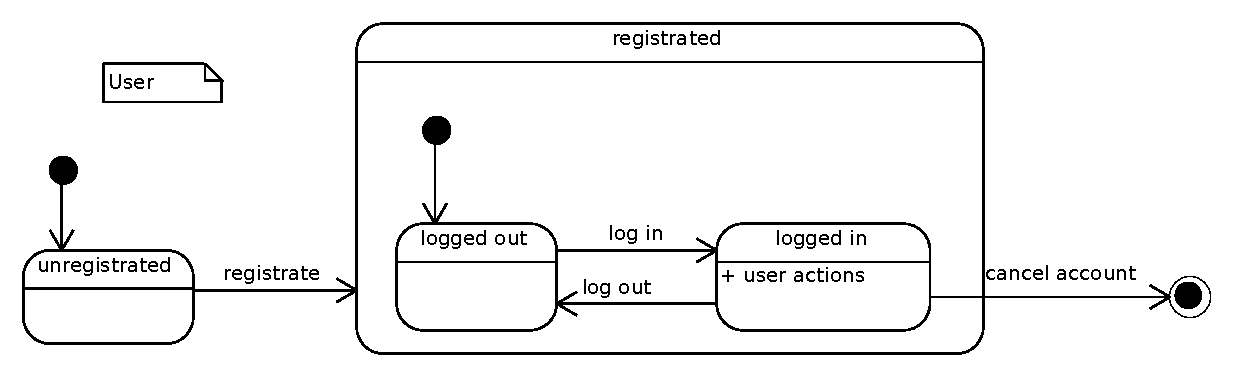
\includegraphics[scale=0.7]{svgs/statechart_user}
\caption{\textit{User's Statechart}.}
\label{fig:statechart_user}
\end{figure}
Possiamo fornire una descrizione dei possibili stati dell'utente in
Figura \vref{fig:statechart_user}: nota che, anche se non è prevista
l'eliminazione da interfaccia grafica di un singolo utente, questa è
sempre possibile andando ad effettuare modifiche nel database. Questa
considerazione può essere valutata anche per le credenziali del Tutore.

\subsubsection{Vista dei Casi d'Uso}
Nella Figura \vref{fig:user_ucview_one} e nella Figura \vref{fig:user_ucview_two} 
mostriamo i primi \textsc{Diagrammi di 
Sequenza} attinenti all'interazione tra Utente ed una generica istanza
del Sistema (\texttt{System}). Questi diagrammi fanno riferimento
ai Casi d'Uso descritti nella Sottosezione \vref{subsec:usecasetext}

\begin{figure}[p]
 \centering
   \subfloat[][\emph{Patient's Registration}.]{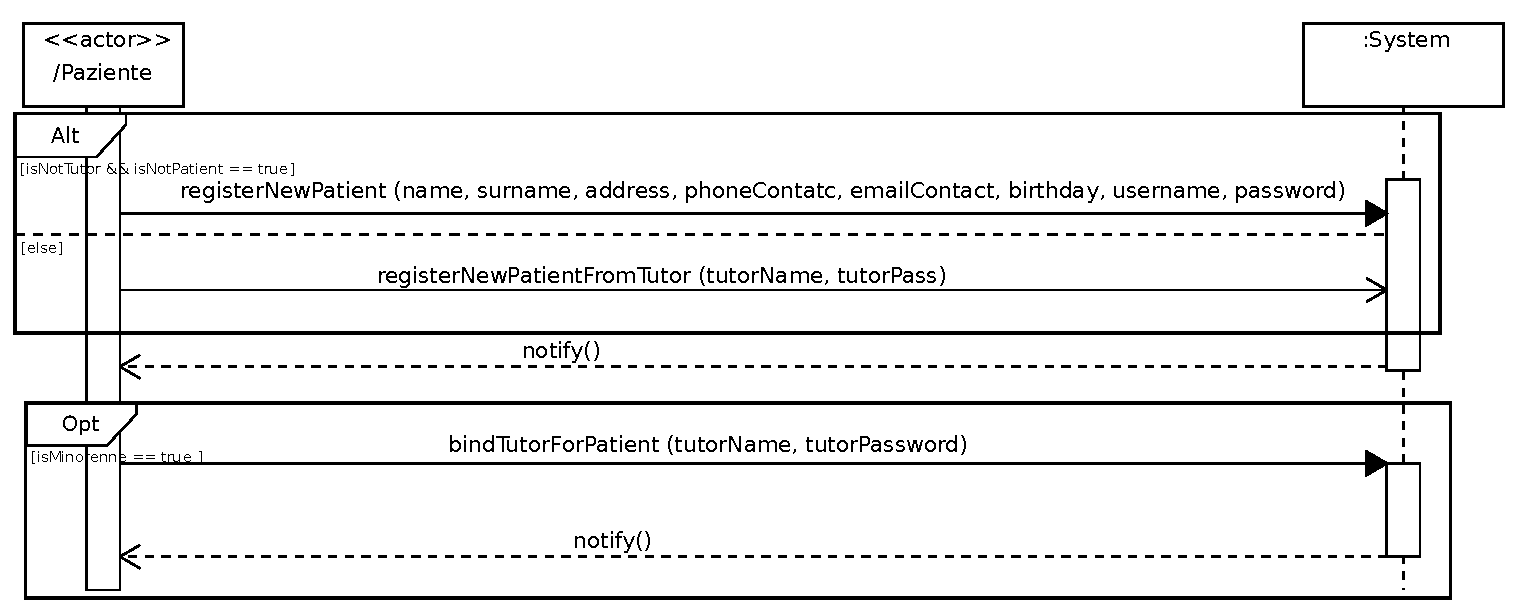
\includegraphics[scale=0.6]{svgs/patient_Registrazionepaziente}}\\
   \subfloat[][\emph{View Reservations}.]{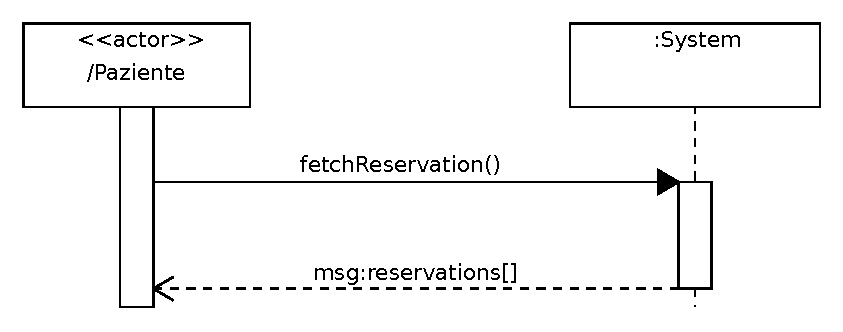
\includegraphics[scale=0.6]{svgs/patient_Visualizzazioneprenotazioni}}
   \subfloat[][\emph{View Reports}.]{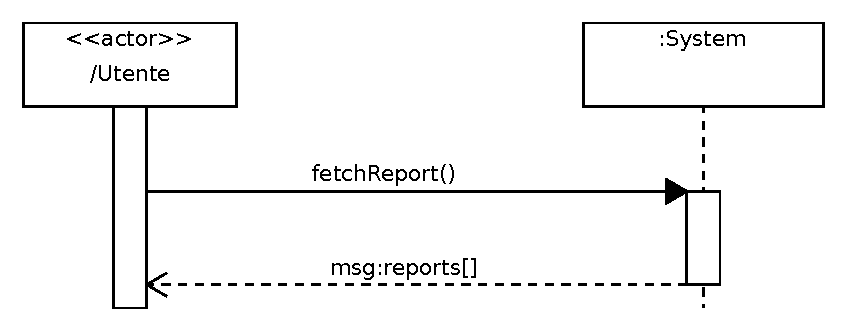
\includegraphics[scale=0.6]{svgs/patient_Visualizzazionereferti}}\\
   \subfloat[][\emph{Request Reservations}.]{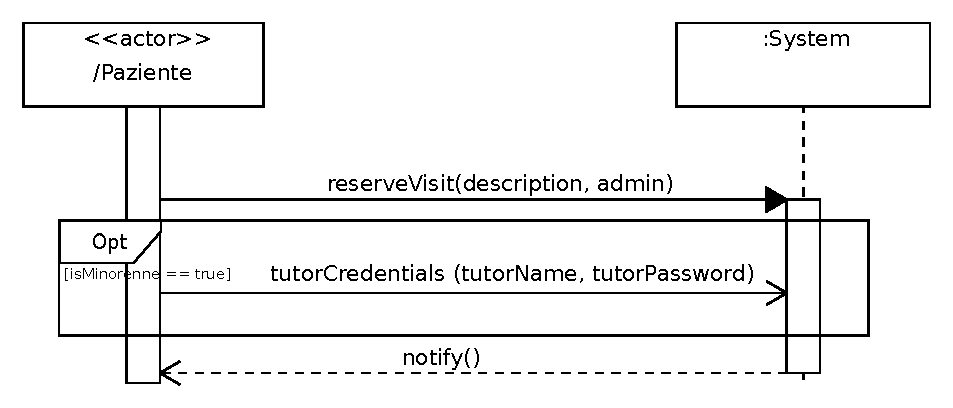
\includegraphics[scale=0.6]{svgs/patient_Effettuareprenotazione}}
   \subfloat[][\emph{User's Login as Patient}.]{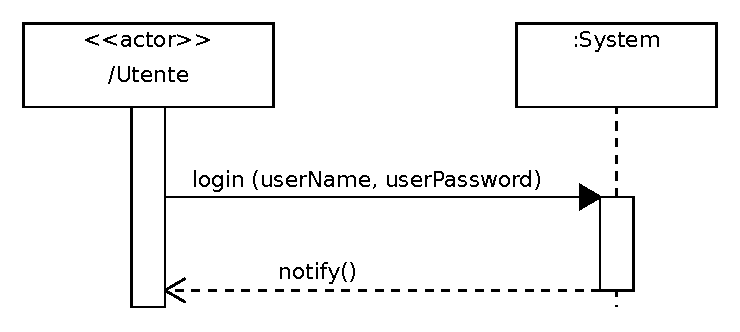
\includegraphics[scale=0.6]{svgs/patient_Loginpaziente}}\\
   \subfloat[][\hbox{\emph{Postpone Patient's Reservation}.}]{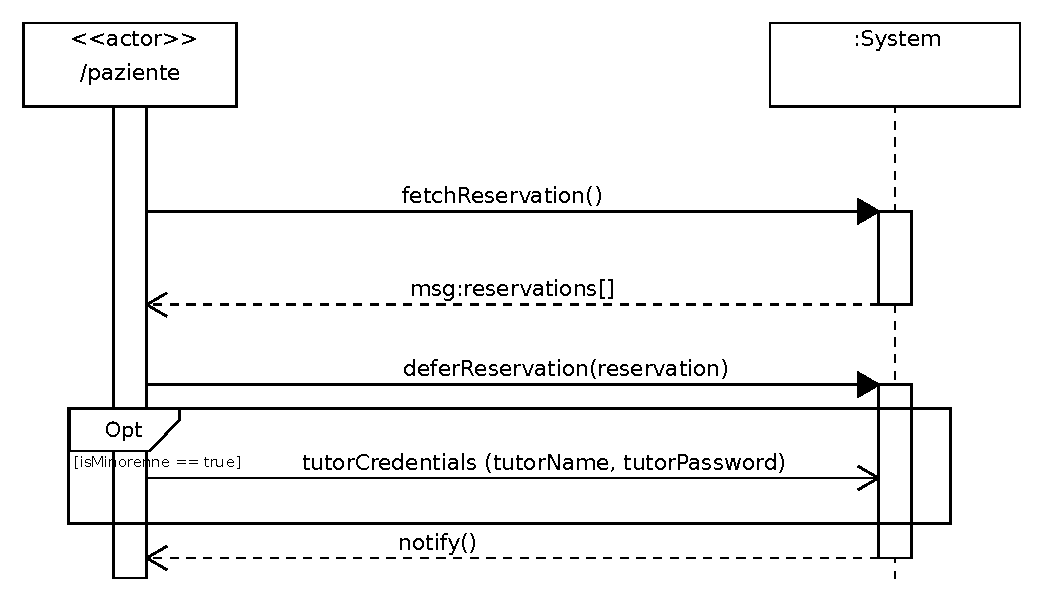
\includegraphics[scale=0.6]{svgs/patient_Posticipoprenotazione}}
   
 \caption{\emph{Users' Use Case View (1)}.}
 \label{fig:user_ucview_one}
\end{figure}

\begin{figure}[!p]
 \centering
   \subfloat[][\hbox{\emph{User's Revoke of Reservation}.}]{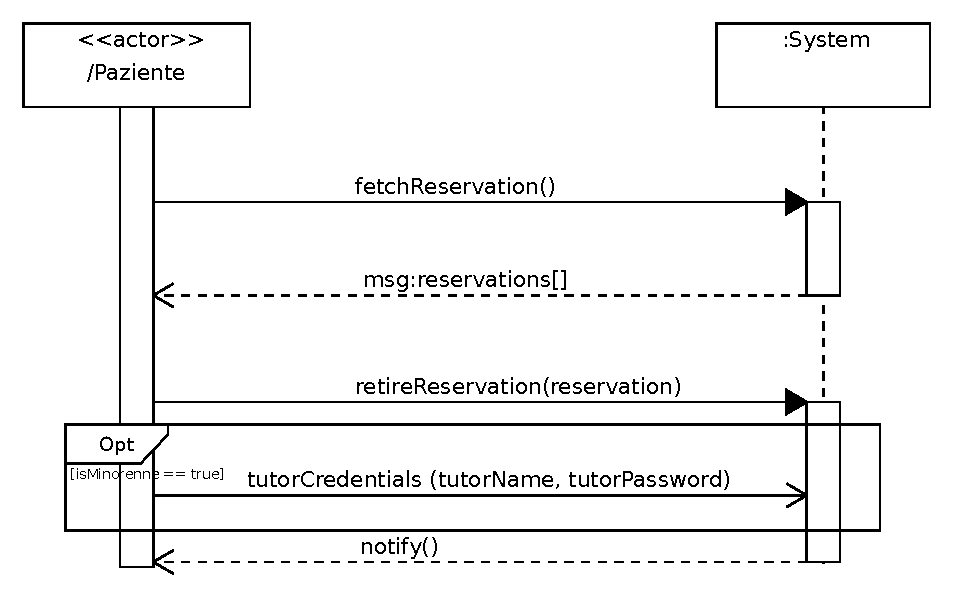
\includegraphics[scale=0.6]{svgs/patient_Annullamentoprenotazione}}\\
   \subfloat[][\hbox{\emph{User's Print}.}]{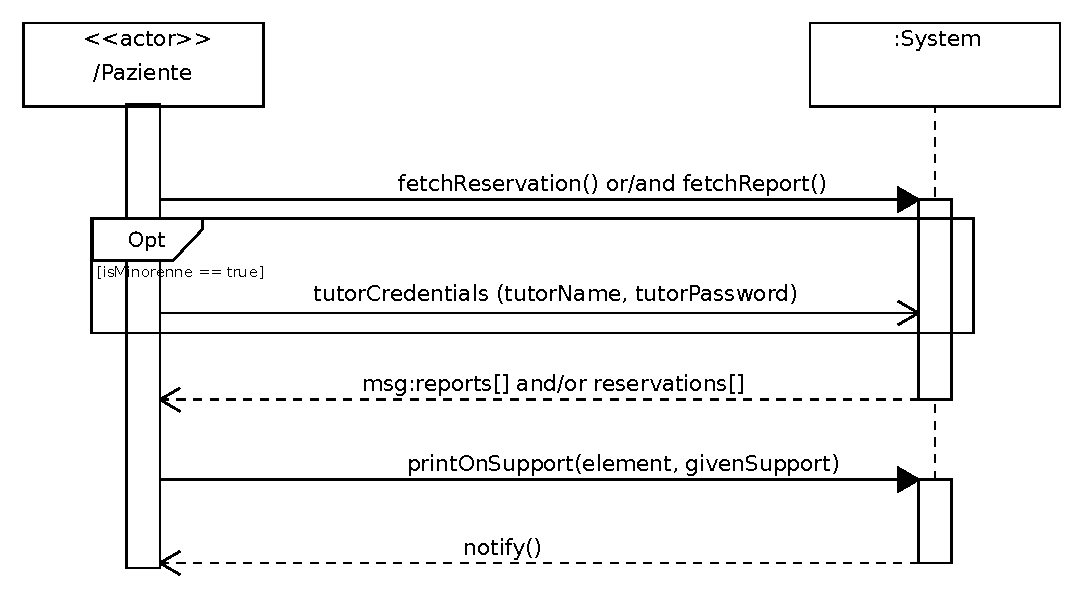
\includegraphics[scale=0.6]{svgs/patient_Stampa}}\\
   \subfloat[][\hbox{\emph{System Methods to implement}.}]{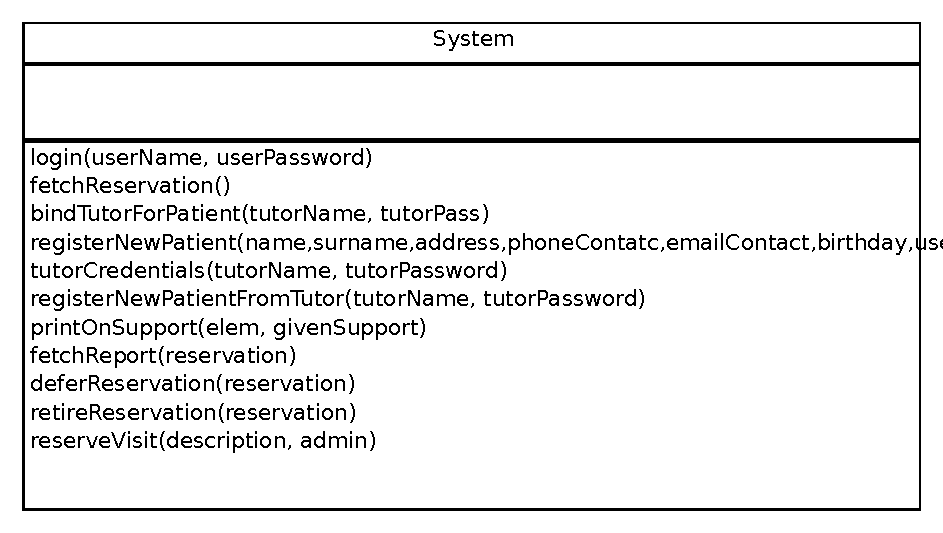
\includegraphics[scale=0.6]{svgs/patient_DiagrammadiClasse}}\\
 \caption{\emph{Users' Use Case View (2)}.}
 \label{fig:user_ucview_two}
\end{figure}

Elenchiamo i contratti che verranno dettagliati più
sotto, allo scopo di definire l'interfaccia 
di sistema pubblica dei nostri metodi:
\begin{itemize}
\diam \texttt{registerNewPatient}
\diam \texttt{login}
\diam \texttt{fetchReservation}
\diam \texttt{fetchReport}
\diam \texttt{tutorCredentials}
\diam \texttt{retireReservation}
\diam \texttt{deferReservation}
\diam \texttt{bindTutorForPatient}
\diam \texttt{printOnSupport}
\diam \texttt{reserveVisit}
\diam \texttt{registerNewPatientFromTutor}
\diam \texttt{registerTutor}
\end{itemize}

\begin{tabularx}{\columnwidth}{cX}
\toprule
\textsc{Contratto 12}:& \textbf{registerNewPatient}\\
\midrule
\textit{Operazione}: & 	\texttt{registerNewPatient(name, surname, address, phoneContatc, emailContact, birthday, username, password)}\\
\textit{Use Case}: &	Registrare il paziente\\
\textit{Pre-condizioni}: &  Nessuna.\\
\textit{Post-condizioni}: & \begin{itemize}
\item Viene inserito un nuovo paziente nel sistema, creando l'elemento $patient$ con i 
rispettivi parametri se il paziente è maggiorenne. (\textit{creazione di istanza})
\end{itemize}\\
\bottomrule
\end{tabularx}
\medskip

\begin{tabularx}{\columnwidth}{cX}
\toprule
\textsc{Contratto 13}:& \textbf{login}\\
\midrule
\textit{Operazione}: & 	\texttt{login(userName, userPassword)}\\
\textit{Use Case}: &	Accedere al sistema.\\
\textit{Pre-condizioni}: &  Nessuna\\
\textit{Post-condizioni}: & \begin{itemize}
\item È stata creata un’istanza $g$ della classe Guest (\textit{creazione di istanza}). 
\item Viene settato lo stato di questa classe come $g.isPatientMinor$ o in 
	$g.isPatientMajor$ a seconda che il paziente sia minorenne o maggiorenne.
\item È settato l'attributo $g.logged$ a $true$ se il paziente è maggiorenne 
	($g.isPatientMajor$) e se l'autenticazione è avvenuta con successo
\end{itemize}\\
\bottomrule
\end{tabularx}
\medskip


\begin{tabularx}{\columnwidth}{cX}
\toprule
\textsc{Contratto 14}:& \textbf{fetchReservation}\\
\midrule
\textit{Operazione}: & 	\texttt{fetchReservation()}\\
\textit{Use Case}: &	Visualizzare lo storico delle prenotazioni\\
\textit{Pre-condizioni}: &  Il paziente è stato autenticato dal sistema\\
\textit{Post-condizioni}: & \begin{itemize}
\item Sono ottenute le istanze delle prenotazioni $reserv[]$ di visita in 
	$patient.reservations$ (\textit{modifica di attributo} ed \textit{associazione
	formata})
\end{itemize}\\
\bottomrule
\end{tabularx}
\medskip

\begin{tabularx}{\columnwidth}{cX}
\toprule
\textsc{Contratto 15}:& \textbf{fetchReport}\\
\midrule
\textit{Operazione}: & 	\texttt{fetchReport(reservation)}\\
\textit{Use Case}: &	Visualizzare lo storico delle prenotazioni\\
\textit{Pre-condizioni}: &  Il paziente è stato autenticato dal sistema ed ha richiesto
di ottenere le prenotazioni.\\
\textit{Post-condizioni}: & \begin{itemize}
\item Ottiene da $reservation$ il referto nell'attributo $reservation.report$
\end{itemize}\\
\bottomrule
\end{tabularx}
\medskip


\begin{tabularx}{\columnwidth}{cX}
\toprule
\textsc{Contratto 16}:& \textbf{tutorCredentials}\\
\midrule
\textit{Operazione}: & 	\texttt{tutorCredentials( tutorName, tutorPassword)}\\
\textit{Use Case}: &	Contattare l’amministratore, Effettuare una prenotazione\\
\textit{Pre-condizioni}: &  L'utente accede in favore di un paziente minorenne.\\
\textit{Post-condizioni}: & \begin{itemize}
\item Si associa al Guest $g$ corrente nell'attributo $tutor$ l'istanza di tutore
	con le credenziali indicate (\textit{associazione formata}).
\end{itemize}\\
\bottomrule
\end{tabularx}
\medskip

\begin{tabularx}{\columnwidth}{cX}
\toprule
\textsc{Contratto 17}:& \textbf{retireReservation}\\
\midrule
\textit{Operazione}: & 	\texttt{retireReservation(res)}\\
\textit{Use Case}: &	Contattare l'amministratore\\
\textit{Pre-condizioni}: &  L'Utente è loggato nel sistema ed ha in precedenza
			effettuato una prenotazione\\
\textit{Post-condizioni}: & \begin{itemize}
\item È creata una nuova istanza di Messagggio $msg$ all'interno del sistema
	(\textit{creazione di istanza})
\item È settata la tipologia di richiesta $msg.kind$ a $revoke$ (\textit{modifica di
	attributo})
\item È associato al messaggio $msg$ la Prenotazione $res$ da revocare
	(\textit{associazione formata})
\item È associato al messaggio $msg$ l'amministratore tramite $msg.destinatario = res.sala.amministratore$
	(\textit{associazione formata})
\item È associato al messaggio $msg$ l'utente $patient$ che ne ha fatto richiesta
	nell'attributo $msg.patient$ (\textit{asociazione formata})
\end{itemize}\\
\bottomrule
\end{tabularx}
\medskip

\begin{tabularx}{\columnwidth}{cX}
\toprule
\textsc{Contratto 18}:& \textbf{deferReservation}\\
\midrule
\textit{Operazione}: & 	\texttt{deferReservation(res)}\\
\textit{Use Case}: &	Contattare l'amministratore\\
\textit{Pre-condizioni}: &  L'Utente è loggato nel sistema ed ha in precedenza
			effettuato una prenotazione\\
\textit{Post-condizioni}: & \begin{itemize}
\item È creata una nuova istanza di Messagggio $msg$ all'interno del sistema
	(\textit{creazione di istanza})
\item È settata la tipologia di richiesta $msg.kind$ a $defer$ (\textit{modifica di
	attributo})
\item È associato al messaggio $msg$ la Prenotazione $res$ da posticipare
	(\textit{associazione formata})
\item È associato al messaggio $msg$ l'amministratore tramite $msg.destinatario = res.sala.amministratore$
	(\textit{associazione formata})
\item È associato al messaggio $msg$ l'utente $patient$ che ne ha fatto richiesta
	nell'attributo $msg.patient$ (\textit{asociazione formata})
\end{itemize}\\
\bottomrule
\end{tabularx}
\medskip


\begin{tabularx}{\columnwidth}{cX}
\toprule
\textsc{Contratto 19}:& \textbf{bindTutorForPatient}\\
\midrule
\textit{Operazione}: & 	\texttt{bindTutorForPatient(tutorName, tutorPassword)}\\
\textit{Use Case}: &	Registrare il paziente\\
\textit{Pre-condizioni}: &  Si richiede la registrazione di un paziente è minorenne\\
\textit{Post-condizioni}: & \begin{itemize}
\item Viene inserito un nuovo paziente nel sistema se la richiesta ha successo, 
	creando l'istanza $patient$ (\textit{creazione di istanza}).
\item A $patient$ vengono associati i parametri forniti precedentemente da
	registerNewPatient (\textit{associazione formata}).
\item Viene associato il $tutor$ indicato da $tutorName$ e $tutorPassword$ 
	al $patient$ nell'attributo $patient.tutor$ (\textit{associazione formata})
\end{itemize}\\
\bottomrule
\end{tabularx}
\medskip

\begin{tabularx}{\columnwidth}{cX}
\toprule
\textsc{Contratto 20}:& \textbf{printOnSupport}\\
\midrule
\textit{Operazione}: & 	\texttt{printOnSupport(element, givenSupport)}\\
\textit{Use Case}: &	Visualizzare lo storico delle prenotazioni\\
\textit{Pre-condizioni}: &  L'utente è autenticato all'interno del sistema e sono 
			presenti delle prenotazione o dei referti ad esse
			associate\\
\textit{Post-condizioni}: & \begin{itemize}
\item Viene richiesto al sistema di stampare il dato referto o la data 
	prenotazione, sul supporto richiesto
\end{itemize}\\
\bottomrule
\end{tabularx}
\medskip


\begin{tabularx}{\columnwidth}{cX}
\toprule
\textsc{Contratto 21}:& \textbf{reserveVisit}\\
\midrule
\textit{Operazione}: & 	\texttt{reserveVisit(description, admin)}\\
\textit{Use Case}: &	Effettuare una prenotazione\\
\textit{Pre-condizioni}: &  Il paziente è autenticato dal sistema\\
\textit{Post-condizioni}: & \begin{itemize}
\item È creata una nuova istanza di Messaggio $msg$ all'interno del sistema
	(\textit{creazione di istanza})
\item È settata la tipologia di richiesta $msg.kind$ a $reserve$ (\textit{modifica di
	attributo})
\item È associato al messaggio $msg$ l'utente $patient$ che ne ha fatto richiesta
	nell'attributo $msg.patient$ (\textit{associazione formata})
\item È associata al messaggio $msg$ una descrizione $description$ sulla richiesta 
	della visita nell'attributo $msg.content$ (\textit{modifica di attributo}).
\item È associato l'amministratore all'interno del messaggio nel campo destinatario:
	$msg.destinatario = admin$
\end{itemize}\\
\bottomrule
\end{tabularx}
\medskip

\begin{tabularx}{\columnwidth}{cX}
\toprule
\textsc{Contratto 22}:&	\textbf{registerNewPatientFromTutor}\\
\midrule
\textit{Operazione}: & 	\texttt{registerNewPatientFromTutor( tutorName, tutorPass)}\\
\textit{Use Case}: &	\texttt{Registrare paziente}\\
\textit{Pre-condizioni}: &
il paziente è presente nel sistema come tutore, ma non come Paziente.\\
\textit{Post-condizioni}: & \begin{itemize}
\item È inserito un nuovo paziente nel sistema (una volta che la richiesta è
	stata accettata), creando l'elemento $patient$ con i parametri forniti 
	dalla registerNewPatientFromTutor.
\end{itemize}\\
\bottomrule
\end{tabularx}
\medskip

\begin{tabularx}{\columnwidth}{cX}
\toprule
\textsc{Contratto 23}:&	\textbf{registerTutor}\\
\midrule
\textit{Operazione}: & 	\texttt{RegisterTutor( tutorName, tutorPass)}\\
\textit{Use Case}: &	\texttt{Registrare paziente}\\
\textit{Pre-condizioni}: & Nessuna\\
\textit{Post-condizioni}: & Viene inserito un nuovo tutor nel sistema, identificato
 dai parametri forniti. Un tutore potrebbe non essere necessariamente un utente 
 del sistema.\\
\bottomrule
\end{tabularx}
\medskip



\subsection{Ampliamenti al modello di dominio suggeriti}
\label{subsubsec:aamddomsugg_admin}
\begin{itemize}
\item È necessario creare una nuova classe \texttt{Slot} che 
contenga gli attributi di \textsc{Data}, \textsc{Ora} e
\textsc{Stanza}.
\item È necessario inserire un attributo \textsc{Prenotazione} all'interno
della classe \texttt{Messaggio}
\item È necessario distinguere i messaggi come \texttt{MPaziente} e \texttt{MAmministratore},
	con \texttt{Messaggio} come loro generalizzazione.
\item È necessario inserire una nuova astrazione tra \textit{Paziente} ed \textit{Amministratore}
detta \texttt{Guest}
\end{itemize}

Ci riserviamo di effettuare queste modifiche nella fase successiva, in quanto
in quel momento, ci appresteremo ad effettuare ulteriori modifiche al modello
di dominio.

\subsection{Definizione delle priorità dei casi d'uso}
Come richiesto dal processo XP, dopo aver attentamente valutato la difficoltà
dei vari casi d'uso, possiamo evidenziare le priorità di implementazione.

\begin{itemize}
\item Come Amministratore, voglio ricevere le richieste di visita in modo da
poter notificare la prenotazione riservata per un paziente ed associarvi
un grado di priorita.

\medskip priorità 10
\bigskip

\item Come Utente, voglio scegliere un reparto in modo da prenotare una
visita associata a quel tipo di servizio medico.

\medskip priorità 9
\bigskip

\item Come Amministratore, voglio visualizzare le prenotazioni in modo da
decidere in quale data effettuare le prenotazioni

\medskip priorità 8
\bigskip

\item Come Utente, voglio essere in grado di registrare me stesso come Paziente
Maggiorenne o come Tutore.

\medskip priorità 6
\bigskip

\item Come Utente, voglio essere in grado di visualizzare le mie prenotazioni
ed eventualmente i referti associati.

\medskip priorità 6

\item Come Tutore, voglio essere in grado di registrare un paziente minorenne
di cui sono responsabile.

\medskip priorità 5
\bigskip

\item Come Amministratore, voglio gestire le prenotazioni in modo da associarvi
o/e modificarvi i referti

\medskip priorità 5
\bigskip
 
\item Come Amministratore, voglio visualizzare le prenotazioni in modo da
ottenere l'insieme delle prenotazioni relativo ad un paziente, ed eventualmente
i referti.

\medskip priorità 5
\bigskip

\item Come Amministratore, voglio poter modificare i reperti medici del paziente.

\medskip priorità 5

\item Come Utente, voglio essere in grado di effettuare l'eliminazione della
prenotazione e di riceverne conferma.

\medskip priorità 5
\bigskip

\item Come Utente, voglio essere in grado di effettuare uno spostamento della
prenotazione gia fissata.


\medskip priorità 5
\bigskip

\item Come Paziente maggiorenne e tutore, voglio ottenere l'autenticazione
allo scopo di ottenere per me o per il mio tutelato i servizi del sistema.

\medskip priorità 4
\bigskip

\item Come Utente, voglio ricevere le notifiche del sistema sulle operazioni di
cancellazione, spostamento, prenotazione richieste all'amministratore.

\medskip priorità 4
\end{itemize}
